\documentclass[sigconf]{acmart}

\usepackage{graphicx}
\usepackage{hyperref}
\usepackage{todonotes}

\usepackage{endfloat}
\renewcommand{\efloatseparator}{\mbox{}} % no new page between figures

\usepackage{booktabs} % For formal tables

\settopmatter{printacmref=false} % Removes citation information below abstract
\renewcommand\footnotetextcopyrightpermission[1]{} % removes footnote with conference information in first column
\pagestyle{plain} % removes running headers

\newcommand{\TODO}[1]{\todo[inline]{#1}}

\begin{document}
\title{Using Big Data to Battle Air Pollution}

\author{Karthik Vegi}
\affiliation{%
  \institution{Indiana University Bloomington}
  \streetaddress{2619 East 2nd Street, Apt 11}
  \city{Bloomington, IN 47401} 
  \country{USA}}
\email{kvegi@iu.com}


% The default list of authors is too long for headers}
\renewcommand{\shortauthors}{kvegi}

\begin{abstract}
We have come a long way from the stone age to build large scale industries, big cities, bullet trains, and a booming automobile industry. Technological and industrial advances are making our cities smarter by the day and yet a nagging side-effect is air pollution. Air pollution is not only creating local health hazards like respiratory and heart problems, but also directly leading to an increase in temperatures and contributing to global warming. We show how the advances in {\em Big Data}, {\em Cloud Computing}, and {\em Internet of Devices} can be used to combat air pollution.
\end{abstract}

\keywords{i523, hid231, big data, environment, air pollution, global warming}

\maketitle

\section{Introduction}
Air pollution is no longer a local problem. It is a global environmental issue which involves individual countries to come together and device measures to combat it \cite{www-ral}. It it causing about 3.7 million premature deaths worldwide from cardiovascular and respiratory diseases and also ruins the crops that feed the world \cite{www-ral}. Air pollution also has a direct effect on a number of environmental issues like global warming, depletion of ozone layer, acid rains, and impacts wild-life \cite{www-ral}. \\
Back in the year 1990, the job of a typical air quality scientist was to develop atmospheric dispersion models to evaluate the air pollution caused by industries and make sure that it is within the permissible level suggested by the {\em Environmental Protection Agency} \cite{www-ibm1}. These models gather historic data of many years from airports and weather balloons to predict the pollution with the help of meteorology theory \cite{www-ibm1}. Although the methods used to derive the values were good enough, the limitations with respect to the technology posed a real challenge which took weeks to run the simulations, only to be cut-off in the middle due to power and storage issues \cite{www-ibm1}. The data processing engine was built on Sun-Solaris workstations with tapes handling the data storage \cite{www-ibm1}. The work-stations set up in major points in the country would communicate using a very slow network connection \cite{www-ibm1}. The data processing would be done locally and later written to all the servers which would then be split and distributed among many machines and consolidated in the end \cite{www-ibm1}. ``If only we had that much more data and that much more ability to handle it, we could iterate through the model at a much finer scale. Real-time data processing remained a pipe dream'' \cite{www-ibm1}. \\

\section{Air Pollution as a Big Data Problem}
The advent of {\em Big Data} and the technological advances changed the way the data is ingested and analyzed \cite{www-ibm1}. The network speeds have increased, wide range of sensors are available to collect data with a lot of precision which would feed the high speed data processing systems. Batch processing has become easier with {\em Hadoop} and {\em Map-Reduce}. The storage mechanisms have become cheaper and more disaster proof. \\
{\em IBM} is helping Beijing combat air pollution by analyzing huge amounts of data using a data analysis platform {\em Green Horizons} \cite{www-huff}. IBM has signed up partnerships with different cities in China and India to deploy {\em Big Data Analytics}, {\em Machine Learning} and {\em Internet of Things} to improve traffic, keep a check on the pollution from industrial machines, and other pollution causing agents \cite{www-huff}. {\em IBM} will deploy sensors in various places to collect data in real-time and analyze previous weather forecasts, and build improved iterative models over time \cite{www-huff}. The system continuously streams data from the sensors and improves the forecast by learning over time using {\em Machine Learning} algorithms \cite{www-huff}. Figure 1 shows the Green Horizons air quality management for Beijing.

\begin{figure}
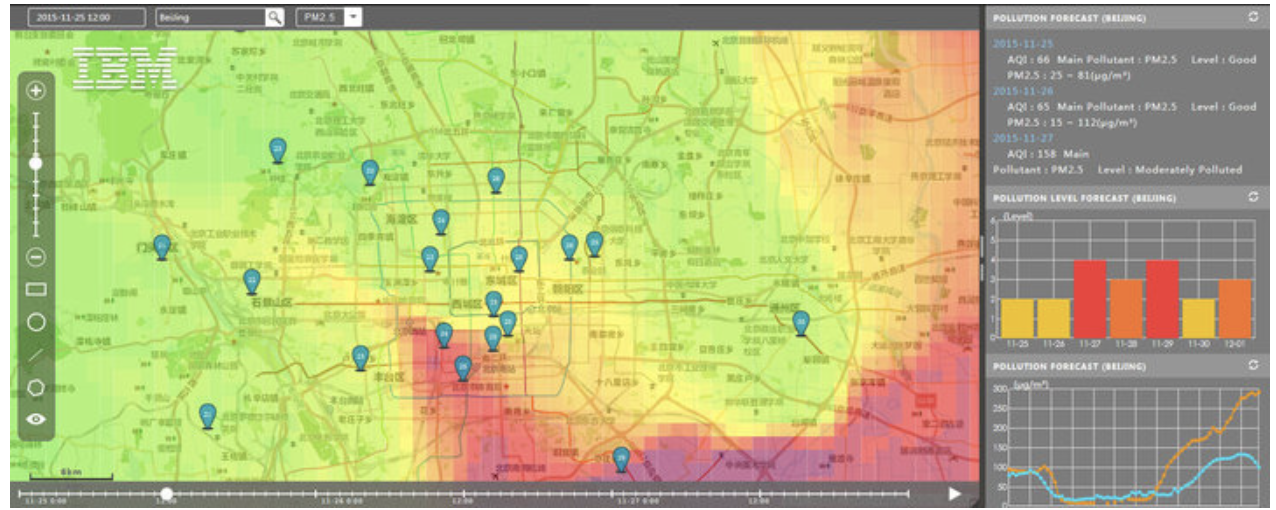
\includegraphics[width=0.7\textwidth]{images/fig1.png}
\caption{Green Horizons air quality management for Beijing \cite{www-huff}}
\end{figure}

{\em IBM} is collaborating with the United Nations to push the use of technological advances by every country for the common good of the world \cite{www-huff}. More and more cities and countries are opening air quality data to public where you can get reports in real time \cite{www-ferro}. The {\em BreezoMeter} is the first mobile application that provides real-time information of the street's air quality information using geo-location maps \cite{www-ferro}. {\em Copernicus} is another monitoring service that ingests data from satellites and on site sensors on land, air and sea to provide continuous information to the users \cite{www-ferro}. {\em Open Data Week} is an intergovernmental organization where 34 states come together to bring reforms and discuss how to use technology and services like {\em Copernicus} that use {\em Big Data} to test prototypes of new products to ensure they operate within the permissible levels of pollution \cite{www-ferro}. \\
While these initiatives help bring awareness about the seriousness of the issue, each state and country should take strict measures to bring out reforms that will help eradicate pollution. {\em Big Data} might never replace the environmental responsibility but it will help to plan the vision for environmental awareness and its tools make it easier to achieve the vision \cite{www-ferro}. These tools can also be used to gauge the alternative sources of energy and the feasibility of tapping into other natural resources ensuring responsible consumption of energy \cite{www-ferro}. For example, {\em IBM Bluemix} analyzed data from a steel industry and the analysis uncovered an interesting insight that the furnace wastes a lot of energy to offset the temperature of the smoke which resulted in optimizing its operation \cite{www-ibm1}.

\section{Big Data Techniques to combat pollution}

\subsection{Random Forest Approach for predicting air quality in Urban Sensing Systems}
Air pollution in an urban setting is very important to monitor because of the population density. Air quality in these areas varies a lot in various parts of the city owing to traffic and presence of industries \cite{raq2016}. A random forest approach ingests data from meteorology, urban sensors, road information, and real-time traffic and predicts the air quality with utmost precision \cite{raq2016}. Real-time air quality information consists of measuring the concentration of $PM_{2.5}$, $PM_{10}$, and $NO_{2}$ \cite{raq2016}. \\
The {\em Air Quality Index} AQI is the measure that is used to understand how polluted the air is \cite{raq2016}. AQI is measured by reading the concentration of 6 pollutant gases namely, sulfur dioxide $SO_{2}$, nitrogen dioxide $NO_{2}$, air particles smaller than 10 $\mu$m $PM_{10}$, air particles smaller than 2.5 $\mu$m $PM_{2.5}$, carbon monoxide $CO$, and ozone $O_3$ \cite{raq2016}. Based on the level of AQI, the air quality is classified as shown in Figure 2. 

\begin{figure}
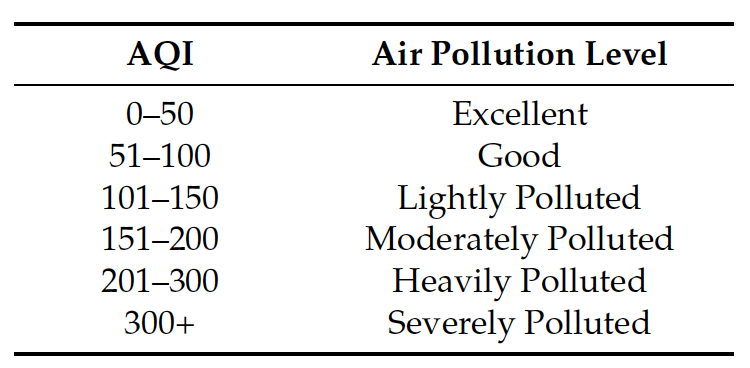
\includegraphics[width=0.5\textwidth]{images/fig2.png}
\caption{AQI classification \cite{raq2016}}
\end{figure}

{\em Traffic Congestion Status} TCS, explains the traffic status at the current hour \cite{raq2016}. Figure 3 shows how colors are used to represent the traffic congestion \cite{raq2016}.

\begin{figure}
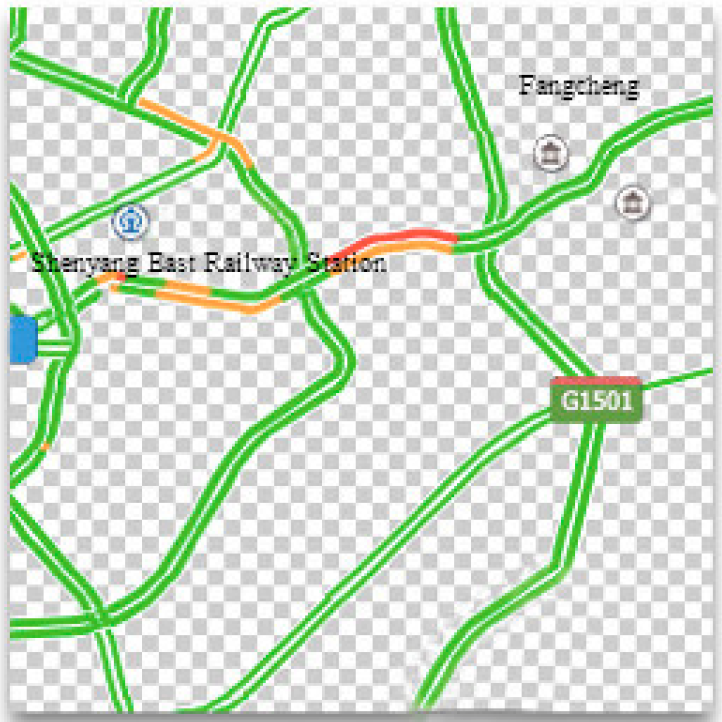
\includegraphics[width=0.4\textwidth]{images/fig3.png}
\caption{Traffic Congestion\cite{raq2016}}
\end{figure}

\subsection{RAQ Algorithm}
The RAQ algorithm collects data from air monitoring station AQI, meteorology data MD, traffic congestion TCS, road information RI, and point of interest POI which is the specific location that someone is interested to visit \cite{raq2016}. The data refresh rate is one hour and the data is collected from different parts of the city which are divided in grids from $G_1$ to $G_n$ \cite{raq2016}. The data is divided into training and testing data sets to train the model and evaluate the model \cite{raq2016}. Figure 4 shows the structure of the data.

\begin{figure}
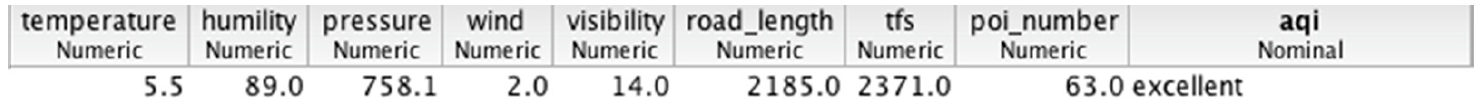
\includegraphics[width=0.7\textwidth]{images/fig4.png}
\caption{Structure of RAQ data\cite{raq2016}}
\end{figure}

A decision tree is used to split and classify the data and the results are aggregated by collecting the data from all the sub-trees \cite{raq2016}. Figure 5 illustrates the procedure of RAQ.

\begin{figure}
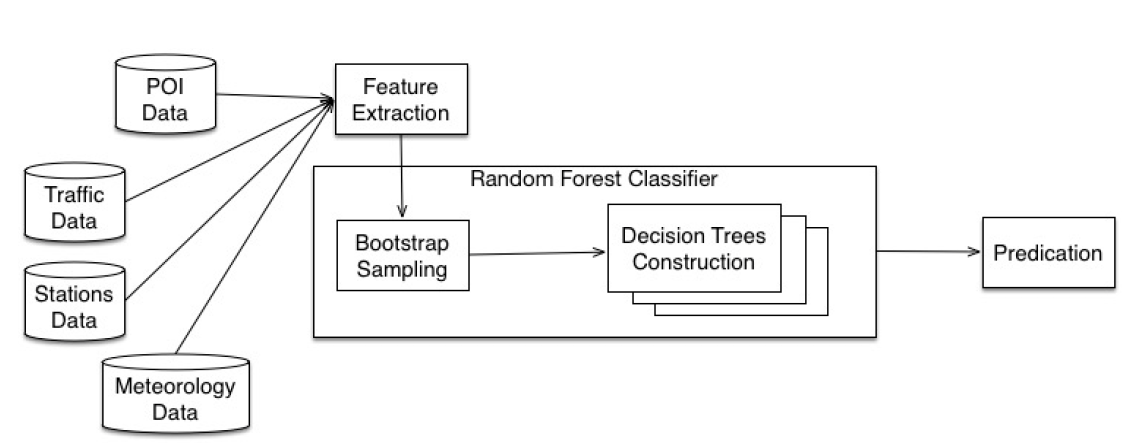
\includegraphics[width=0.5\textwidth]{images/fig5.png}
\caption{Procedure of RAQ \cite{raq2016}}
\end{figure}

The {\em Random Forest} algorithm is employed using the tree type classifier to recursively partition the dataset and generate sub-trees and finally aggregate the results of each sub-tree \cite{raq2016}. Each sub-tress is constructed using {\em Bootstrap Aggregating} where each data set is divided into different buckets by using statistical samples \cite{raq2016}. Once the trees are constructed, each subset of data is fed into a decision tree and the estimated AQI index is calculated \cite{raq2016}. The final AQI index is determined as the maximum value out of all the individual values \cite{raq2016}. Figure 6 shows the step-by-step RAQ algorithm.

\begin{figure}
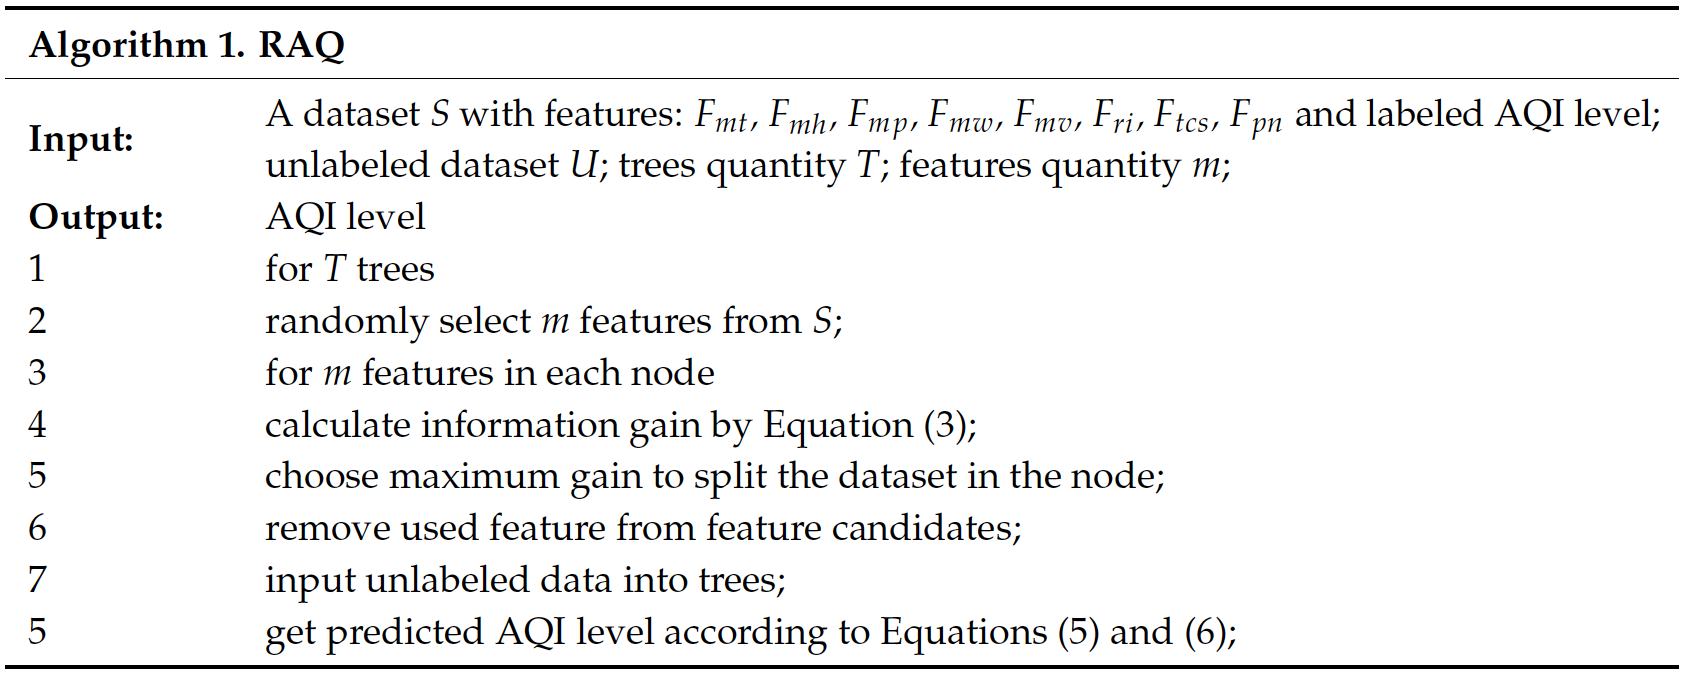
\includegraphics[width=0.5\textwidth]{images/fig6.png}
\caption{RAQ Algorithm \cite{raq2016}}
\end{figure}

\section{Machine Learning models}
{\em Machine Learning} deals with augmenting computers with the ability to learn from data and program themselves \cite{gagan2017}. These algorithms can be used to evaluate the air quality \cite{gagan2017}. 

\subsection{Artificial Neural Network Model}
Artificial Neural Network Model tries to solve the problem by simulating the functioning of brain and neurons \cite{gagan2017}. The model architecture is a function of a sigmoid \cite{gagan2017}. For this experiment, the air quality data was divided into training, test, and validation data with  split of 60, 20, and 20 with a back propagation network of two hidden layers \cite{gagan2017}. To ensure consistency, the air quality data for the training and test sets are derived from the same season \cite{gagan2017}. The air quality is forecast by looking at the historic data where the input and output are represented by the air quality data measured at different times \cite{gagan2017}. The model turns out to be reliable with a good prediction accuracy with the lowest mean square error of $3.7 \times 10^{-4}$ \cite{gagan2017}. The Artificial Neural Network Model is combined with {\em Markov Chains} to develop a new improved model with improved prediction accuracy where the ANN computes the primary values and the results are re-computed and improved by the markov transitional probability matrices \cite{gagan2017}. Figure 7 shows the Artificial Neural Network Model with two hidden layers. 

\begin{figure}
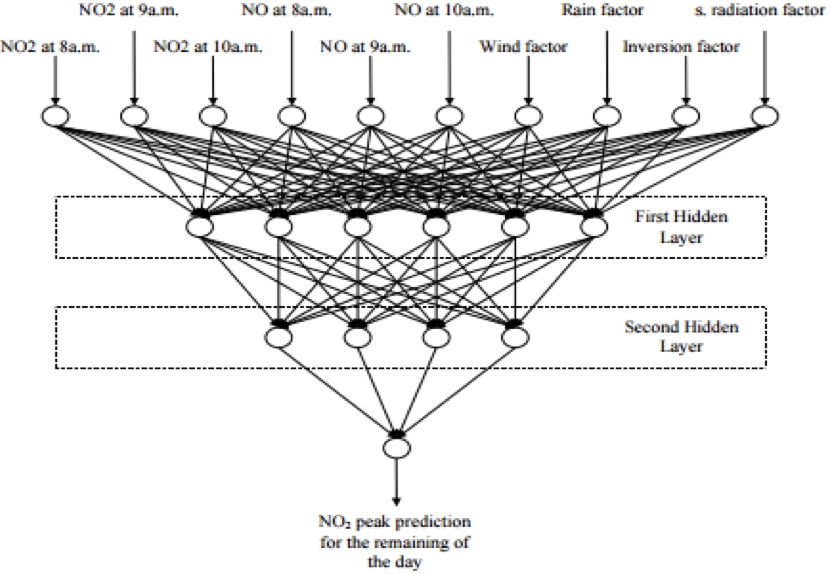
\includegraphics[width=0.5\textwidth]{images/fig7.png}
\caption{Artificial Neural Network(ANN) Model \cite{gagan2017}}
\end{figure}

\subsection{Least squares Support Vector Machine Model}
Least squares support vector machine is a supervised learning model used for classification and regression analysis which arrives at the solution by solving the data represented in the form of linear equations \cite{gagan2017}. For this model, the sample data was collected from 100 sensor points in different intervals of time and at different geographical locations that ranged from urban areas with population, areas near the airport, water surface areas like lakes, and sewage processing areas \cite{gagan2017}. The sample data was a good split with 80 percent collected from urban sewage area and the other data collected from air surface areas \cite{gagan2017}. The fluorescence content in the air was analyzed by a portable air quality measuring device developed in-house by Zhejiang University \cite{gagan2017}. The fluorescence data captured using the device is highly dimensional and non-linear and therefore data pre-processing is essential to bring the dimensions down to a manageable level \cite{gagan2017}. This eliminates the ambient noise and the temperature drift from the data \cite{gagan2017}. The algorithm predicts the regression model by looking at the training data for each cluster \cite{gagan2017}. Finally, the vector consine distance is used to classify the sample into clusters and the performance criterion such as {\em Root Mean Square Error}  and {\em Mean Absolute Error} are computed which demonstrate the efficiency of the algorithm \cite{gagan2017}. Figure 8 shows the pictorial representation of the algorithm.

\begin{figure}
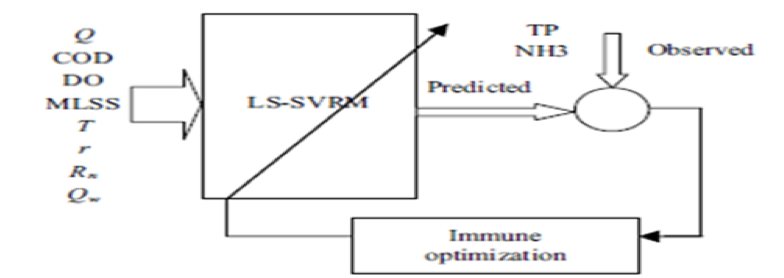
\includegraphics[width=0.5\textwidth]{images/fig8.png}
\caption{Least squares Support Vector Machine Model \cite{gagan2017}}
\end{figure}

\section{Conclusion}
While the new age technologies have a big role to play in measuring, tracking, and keeping air pollution in check, each person should have individual environmental responsibility to make the world a better place to live in. {\em Internet of Things} and {\em Machine Learning} are augmenting the {\em Big Data} capabilities like never before. This ensures that we have more data points to work in a given time and continuous data streaming means more accurate real-time analytics with efficient {\em Machine Learning} algorithms. All these three technologies will continue to work in tandem to keep a check on air pollution and the imminent threats.

\begin{acks}

The author would like to thank Dr. Gregor von Laszewski and the teaching assistants for their support and suggestions.

\end{acks}

\bibliographystyle{ACM-Reference-Format}
\bibliography{report} 

\end{document}
